\newcommand{\chapter}[2][]{
	\newcommand{\chapname}{#2}
	\begin{flushleft}
		\begin{minipage}[t]{\linewidth}
			
\includegraphics[height=1cm]{hdht-logo.png}
			\hspace{0pt}	
			\sffamily\bfseries\large Bài  4 + Bài 5.
			\begin{flushleft}
				\LARGE\bfseries #1
			\end{flushleft}
		\end{minipage}
	\end{flushleft}
	\vspace{1cm}
	\normalfont\normalsize
}
\chapter[Mô tả chuyển động:\\Độ dịch chuyển và quãng đường đi được \\Tốc độ và vận tốc]{Mô tả chuyển động: \\Độ dịch chuyển và quãng đường đi được \\ Tốc độ và vận tốc}
\section{Lý thuyết}
\subsection{Chuyển động cơ. Chất điểm}
\subsubsection{Chuyển động cơ}
Chuyển động cơ của một vật (gọi tắt là chuyển động) là sự thay đổi vị trí của vật đó so với các vật khác theo thời gian.
\subsubsection{Chất điểm}
Một vật chuyển động được coi là một chất điểm nếu kích thước của nó rất nhỏ so với độ dài đường đi (hoặc so với những khoảng cách mà ta đề cập đến).

Ví dụ: trong chuyển động của ôtô từ thành phố Hồ Chí Minh đến Hà Nội thì ôtô được xem là chất điểm.
\subsubsection{Quỹ đạo}
Tập hợp tất cả các vị trí của một chất điểm chuyển động tạo ra một đường trong không gian, đường đó gọi là quỹ đạo của chuyển động.
\subsection{Cách xác định vị trí của vật trong không gian}
\subsubsection{Vật làm mốc và thước đo}
Nếu đã biết đường đi (quỹ đạo) của vật, ta cần chọn một vật làm mốc và một chiều dương trên đường đi, và dùng thước đo chiều dài đoạn đường từ vật làm mốc đến vật là có thể xác định được chính xác vị trí của vật.
\begin{center}
	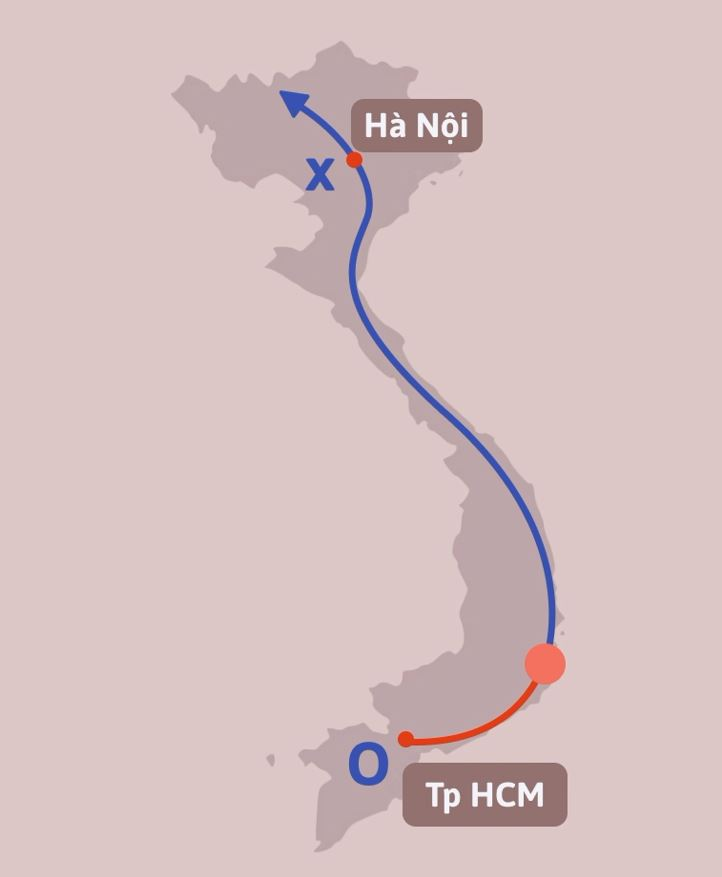
\includegraphics[scale=0.3]{../figs/VN10-PH-02-L-001-1-V2-01.jpg}
\end{center}
\subsubsection{Hệ tọa độ}
Muốn xác định vị trí của một điểm trên một mặt phẳng ta cần có hệ tọa độ với hai trục O$x$ và O$y$ vuông góc nhau, hình chiếu vuông góc của điểm xuống hai trục tọa độ đó chính là tọa độ của điểm đó.
\begin{center}
	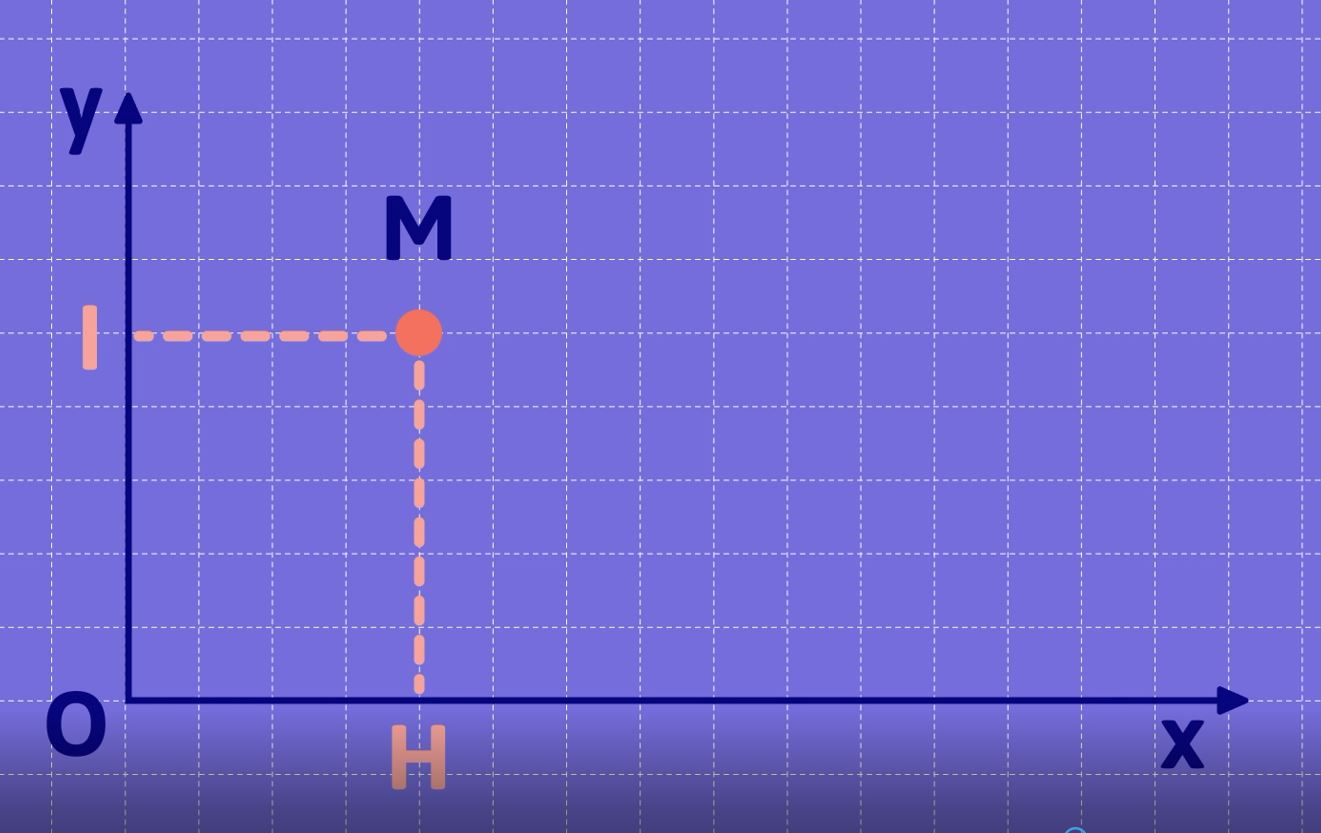
\includegraphics[height=3cm]{../figs/VN10-PH-02-L-001-1-V2-02.jpg}
\end{center}
\subsection{Cách xác định thời gian trong chuyển động}
\subsubsection{Mốc thời gian và đồng hồ}
Để mô tả chuyển động của một vật ta phải biết tọa độ của vật đó ở những thời điểm khác nhau. Muốn thế, ta phải chỉ rõ mốc thời gian và đo khoảng thời gian trôi đi kể từ mốc thời gian bằng một đồng hồ.
\subsubsection{Thời điểm và thời gian}
Nếu lấy mốc thời gian là thời điểm vật bắt đầu chuyển động (thời điểm 0) thì số chỉ của thời điểm sẽ trùng với số đo khoảng thời gian đã trôi qua kể từ mốc thời gian.
\subsection{Hệ quy chiếu}
Một hệ quy chiếu gồm:
\begin{itemize}
	\item mốc tọa độ và một hệ tọa độ để đo vị trí;
	\item mốc thời gian và một đồng hồ để đo thời điểm.
\end{itemize}
\subsection{Quãng đường đi được trong chuyển động thẳng đều}
Trong chuyển động thẳng đều, quãng đường đi được $s$ tỉ lệ với thời gian chuyển động $t$:
\begin{equation*}
	s=vt,
\end{equation*}
trong đó, $v$ là tốc độ của vật.
\subsection{Phương trình chuyển động thẳng đều}
Xét một chất điểm chuyển động thẳng đều trên đường thẳng O$x$ với tốc độ $v$. Ở thời điểm ban đầu ($t_0=0$), vật ở vị trí A cách gốc O một đoạn $x_0$. Vào thời điểm $t$, vật ở vị trí M cách gốc O một đoạn $x$.  
	\begin{center}
	\begin{tikzpicture}
		\coordinate (O) at (0,0);
		\coordinate (A) at (2,0);
		\coordinate (M) at (5,0);
		\coordinate (x) at (8,0);
		\coordinate (O1) at ($(O)-(0,1cm)$);
		\coordinate (A1) at ($(A)-(0,1cm)$);
		\draw[->,thick] (O) -- (x);
		\foreach \i in {O,A}{
			\filldraw[black] (\i) circle (0.5mm);
		}
		\node[label=90:O] at (O){};	
		\node[label=90:A] at (A){};
		\node[label=90:M] at (M){};	
		\node[label=90:x] at (x){};	
		\draw[<->] (O1) -- (A1);
		\node [fill=white] (F1) at ($(O1)!0.5!(A1)$) {$x_0$};
		\coordinate (M1) at ($(M)-(0,1cm)$);
		\draw[<->] (A1) -- (M1);
		\node [fill=white] (F2) at ($(A1)!0.5!(M1)$) {$s$};
		\coordinate (O2) at ($(O)-(0,1.5cm)$);
		\coordinate (M2) at ($(M)-(0,1.5cm)$);
		\draw[<->] (O2) -- (M2);
		\node [fill=white] (F3) at ($(O2)!0.5!(M2)$) {$x$};
		\draw[dashed] (O) -- (O2);
		\draw[dashed] (A) -- (A1);
		\draw[dashed] (M) -- (M2);
		\filldraw[blue] (M) circle (0.5mm);
		%		\node[above of=O]()
	\end{tikzpicture}
\end{center}

Tọa độ của chất điểm sau thời gian chuyển động $t$ là:
\begin{equation}
	x=x_0+s=x_0+vt.
\end{equation}

Phương trình dùng để xác định tọa độ của M theo thời gian được gọi là phương trình chuyển động của chất điểm M. Trong trường hợp này, M chuyển động thẳng đều nên phương trình này gọi là phương trình chuyển động thẳng đều của điểm M. 
\subsubsection{Tốc độ trung bình}
Tốc độ trung bình $v_{\text{tb}}$ là đại lượng đặc trưng cho mức độ nhanh hay chậm của chuyển động; được đo bằng thương số giữa quãng đường đi được $s$ và khoảng thời gian $t$ để đi hết quãng đường đó:
\begin{equation}
	v_{\text{tb}}=\dfrac{s}{t}.
\end{equation}
Trong hệ SI, đơn vị của tốc độ trung bình là m/s. Các đơn vị khác cũng thường được sử dụng là km/h, cm/s...
\subsubsection{Chuyển động thẳng đều}
Chuyển động thẳng đều là chuyển động có quỹ đạo là \bltext{đường thẳng} và có tốc độ trung bình \bltext{như nhau} trên mọi quãng đường ($v_{\text{tb}}\equiv v$).	

\section{Mục tiêu bài học - Ví dụ minh họa}
\begin{dang}{Thực hiện xác định thời điểm và thời gian (mốc thời gian và đồng hồ)}
	\viduii{2}{Giờ Berlin chậm hơn giờ Hà Nội 5 giờ. Trận bóng đá diễn ra tại Beclin lúc 19h00 ngày 2-9-2021. Khi đó theo giờ Hà Nội là
		\begin{mcq}(2)
			\item 14h00 ngày 3-9-2021.
			\item 0h00 ngày 3-9-2021. 
			\item 0h00 ngày 2-9-2021
			\item 14h00 ngày 2-9-2021.
		\end{mcq}
	}
	{	\begin{center}
			\textbf{Hướng dẫn giải}
		\end{center}
		
		Giờ Berlin chậm hơn giờ Hà Nội 6 giờ, nghĩa là
		$$t_{\text{B}}+\SI{6}{\hour}=t_{\text{HN}}.$$
		Trận bóng đá diễn ra tại Berlin lúc 19h00 ngày 2-9-2007. Thời điểm đó theo giờ Hà Nội là:
		$$t_{\text{HN}}=t_{\text{B}}+\SI{6}{\hour}=19\text{h}00 + 6\text{h} = 25\text{h}00 = \SI{24}{\hour}+\SI{1}{\hour}.$$
		Một ngày chỉ có 24 giờ nên thời điểm trên đã bước sang ngày hôm sau. Do đó, trận bóng trên diễn ra vào lúc 1h00 ngày 3-9-2007 giờ Hà Nội. 	
		
		\textbf{Đáp án: B}.
	}
	\viduii{3}{Theo lịch trình tại bến xe ở Hà Nội thì ô tô chở khách trên tuyến Hà Nội - Hải Phòng chạy từ Hà Nội lúc 6 giờ sáng, đi qua Hải Dương lúc 7 giờ 15 phút sáng và tới Hải Phòng lúc 8 giờ 50 phút sáng cùng ngày. Hà Nội cách Hải Dương 60 km và cách Hải Phòng $\SI{105}{km}$. Xe ô tô chạy liên tục không nghỉ dọc đường, chỉ dừng lại 10 phút tại bến xe Hải Dương để đón, trả khách. Tính khoảng thời gian chuyển động và quãng đường đi được của các hành khách sau:
		\begin{enumerate}[label=\alph*)]
			\item Hành khách lên xe tại Hà Nội đi Hải Phòng.
			\item Hành khách lên xe tại Hải Dương đi Hải Phòng.
		\end{enumerate}
	}
	{	\begin{center}
			\textbf{Hướng dẫn giải}
		\end{center}
		
		\begin{enumerate}[label=\alph*)]
			\item Đối với hành khách lên xe tại Hà Nội đi Hải Phòng, chọn bến xe Hà Nội làm mốc và thời điểm ô tô bắt đầu xuất phát là mốc thời gian.
			
			Khoảng thời gian chuyển động là:	
			\begin{center}
				(8 giờ 50 phút - 6 giờ) - 10 phút = 2 giờ 40 phút.
			\end{center}
			Quãng đường đi được đúng bằng độ dài của đoạn đường Hà Nội - Hải Phòng là $\SI{105}{km}$.
			\item Đối với hành khách lên xe tại Hải Dương đi Hải Phòng, chọn bến xe Hải Dương làm mốc và thời điểm ô tô bắt đầu xuất phát là mốc thời gian.
			
			Khoảng thời gian chuyển động là:
			\begin{center}
				8 giờ 50 phút - (7 giờ 15 phút + 10 phút) = 1 giờ 25 phút.
			\end{center}
			Quãng đường đi được là:
			$$\SI{105}{km}-\SI{60}{km}=\SI{45}{km}.$$
		\end{enumerate}
	}
\end{dang}
\begin{dang}{Xác định quãng đường, vận tốc \\trong chuyển động thẳng đều}
	\viduii{3}{Một ô tô đi trên con đường bằng phẳng với $v = \SI{60}{km/h}$, trong thời gian 5 phút, sau đó lên dốc 3 phút với $v = \SI{40}{km/h}$. Coi ôtô chuyển động thẳng đều. Tính quãng đường ô tô đã đi trong cả giai đoạn.
	}
	{	\begin{center}
			\textbf{Hướng dẫn giải}
		\end{center}
		
	Quãng đường ô tô đi được trên đoạn đường phẳng
	$$s_1 =v_1t_1 =\xsi{60}{\kilo\meter/\hour}\cdot\xsi{5}{\minute}=\dfrac{\xsi{60}{\kilo\meter}}{\xsi{1}{\hour}}\cdot\xsi{5}{\minute}=\dfrac{\xsi{60}{\kilo\meter}}{\xsi{60}{\minute}}\cdot\xsi{5}{\minute}=\SI{5}{km}.$$
	
	Quãng đường ô tô lên dốc
	$$s_2 = v_2t_2=\xsi{40}{\kilo\meter/\hour}\cdot\xsi{3}{\minute}=\dfrac{\xsi{40}{\kilo\meter}}{\xsi{1}{\hour}}\cdot\xsi{3}{\minute}=\dfrac{\xsi{40}{\kilo\meter}}{\xsi{60}{\minute}}\cdot\xsi{3}{\minute} = \SI{2}{km}.$$
	
	Quãng đường ô tô đã đi trong cả giai đoạn
	$$s = s_1+s_2 = \SI{7}{km}.$$
		
	}
	\viduii{3}{Hai xe cùng chuyển động đều trên đường thẳng. Nếu chúng đi ngược chiều thì cứ 30 phút khoảng cách của chúng giảm $\SI{40}{km}$. Nếu chúng đi cùng chiều thì cứ sau 20 phút khoảng cách giữa chúng giảm $\SI{8}{km}$. Tính vận tốc mỗi xe.
	}
	{	\begin{center}
			\textbf{Hướng dẫn giải}
		\end{center}
		
		Nếu đi ngược chiều thì 
		\begin{align}
			s_1+s_2 =(v_1+v_2)t_1 &=\xsi{40}{\kilo\meter}\nonumber\\
			\Rightarrow\qquad v_1+v_2&=\dfrac{\xsi{40}{\kilo\meter}}{\xsi{0.5}{\hour}}=\xsi{80}{\kilo\meter/\hour}\label{eq:tongv}
		\end{align}
		Nếu đi cùng chiều thì	
		\begin{align}
			s'_1-s'_2 =(v_1-v_2)t_2 &=\xsi{8}{\kilo\meter}\nonumber\\
			\Rightarrow\qquad v_1-v_2&=\dfrac{\xsi{8}{\kilo\meter}}{\xsi{\frac{1}{3}}{\hour}}=\xsi{24}{\kilo\meter/\hour}\label{eq:hieuv}
		\end{align}
		
		Giải hệ gồm 2 phương trình \eqref{eq:tongv} và \eqref{eq:hieuv}, ta tìm được:
		$$v_1 = \SI{52}{km/h};\quad v_2 =\SI{28}{km/h}.$$
		
		\luuy{Khi làm bài, ta cần phải đổi các đại lượng cùng loại về cùng một đơn vị.\\Ví dụ, trong bài này, ta phải đổi tất cả thời gian về cùng một đơn vị là giờ (h).}
		
		
	}
\end{dang}
\begin{dang}{Xây dựng phương trình, tính các đại lượng\\ trong phương trình chuyển động thẳng đều\\ cho một hoặc hai vật.}
	\viduii{3}{	Trên đường thẳng từ nhà đến chỗ làm việc của A, cùng một lúc xe 1 khởi hành từ nhà đến chỗ làm với $v_1=\SI{80}{\km/\hour}$. Xe 2 từ chỗ làm đi cùng chiều xe 1 với $v_2=\SI{60}{\km/\hour}$. Biết quãng đường từ nhà đến chỗ làm là $\SI{40}{\km}$. Lập phương trình chuyển động của mỗi xe với cùng hệ quy chiếu.
	}
	{	\begin{center}
			\textbf{Hướng dẫn giải}
		\end{center}
		
		Chọn hệ quy chiếu gồm:
		\begin{itemize}
			\item Chiều dương cùng chiều với chiều chuyển động với hai xe;
			\item Gốc tọa độ tại A;
			\item Mốc thời gian lúc hai xe bắt đầu xuất phát.
		\end{itemize}
		
		Xe 1 có phương trình chuyển động
		\begin{equation*}
			x_1=x_0 + v_1t = 80t\textrm{ (km, h)}.
		\end{equation*}
		Xe 2 có phương trình chuyển động  
		\begin{equation*}
			x_2=x_0 + v_2t = 40+60t\textrm{ (km, h)}.
		\end{equation*}
	}
	\viduii{3}{	Hai vật chuyển động ngược chiều qua A và B cùng một lúc. Vật qua A có vận tốc $v_1=\SI{10}{\meter/\second}$, vật qua B có vận tốc $v_2=\SI{15}{\meter/\second}$. Cho biết AB có chiều dài $\SI{100}{m}$.Lấy trục tọa độ là đường thẳng AB, gốc tọa độ ở B, chiều dương từ A sang B, mốc thời gian là lúc chúng cùng qua A và B. Lập phương trình chuyển động của mỗi vật.
	}
	{	\begin{center}
			\textbf{Hướng dẫn giải}
		\end{center}
		
		
		Hệ quy chiếu gồm:
		\begin{itemize}
			\item Chiều dương từ A sang B;
			\item Gốc tọa độ tại B;
			\item Mốc thời gian lúc hai vật cùng qua A và B.
		\end{itemize}
		
		Phương trình chuyển động của vật qua A là
		\begin{equation*}
			x_\text{A}=x_{0\text{A}} + v_\text{A}t =-100+10t\textrm{ (m, s)}.
		\end{equation*}
		
		Phương trình chuyển động của vật qua B là
		\begin{equation*}
			x_\text{B}=x_{0\text{B}} + v_\text{B}t = -15t\textrm{ (m, s)}.
		\end{equation*}
		
	}
\end{dang}

\begin{dang}{Xác định vị trí, thời điểm \\hai vật chuyển động thẳng đều gặp nhau}
	\viduii{3}{	Hai vật chuyển động ngược chiều qua A và B cùng một lúc. Vật qua A có vận tốc $v_1=\SI{10}{\meter/\second}$, vật qua B có vận tốc $v_2=\SI{15}{\meter/\second}$. Cho biết AB có chiều dài $\SI{100}{m}$. Xác định vị trí và thời điểm chúng gặp nhau.
		
	}
	{	\begin{center}
			\textbf{Hướng dẫn giải}
		\end{center}
		Chọn gốc tọa độ ở vị trí B, gốc thời gian ở thời điểm hai vật đang ở A và B. 
		Hai vật gặp nhau khi chúng có cùng tọa độ
		\begin{equation*}
			x_\text{1}=x_\text{2}\Rightarrow -100+10t=-15t \Rightarrow t=\SI{4}{\second}.
		\end{equation*}
		Dựa vào phương trình chuyển động, ta xác định được vị trí hai vật gặp nhau 
		\begin{equation*}
			x_\text{1}=x_\text{2}=v_\text{2}t=\SI{-15}{\meter/\second}\cdot\SI{4}{\second}=\SI{-60}{\meter}.
		\end{equation*}
	}
	\viduii{3}{Lúc 7 giờ, một người ở A chuyển động thẳng đều với $ v= \SI{36}{km/h}$ đuổi theo người ở B đang chuyển động với $v = \SI{5}{m/s}$. Biết $AB = \SI{18}{km}$. Viết phương trình chuyển động của 2 người. Hai người đuổi kịp nhau tại nơi cách A một khoảng 
		\begin{mcq}(4)
			\item $\SI{58}{km}$.
			\item $\SI{46}{km}$.
			\item $\SI{36}{km}$.
			\item $\SI{24}{km}$.
		\end{mcq}
	}
	{	\begin{center}
			\textbf{Hướng dẫn giải}
		\end{center}
		
		Chọn gốc toạ độ tại A, gốc thời gian lúc 7 giờ.
		
		Phương trình chuyển động của hai người ở A và B lần lượt có dạng 
			\begin{align*}
				x_\text{A} &= 36t;\\
				x_\text{B} &=x_0+v_\text{B}t=18+18t.
			\end{align*}
		
		Khi hai người gặp nhau, tọa độ của hai người trùng nhau  
			\begin{align*}
				x_1&=x_2 \quad
				\Rightarrow\quad 36t=18+18t\quad\Rightarrow\quad t=\SI{1}{h}
			\end{align*}
		
		Dựa vào phương trình chuyển động, suy ra nơi gặp nhau cách A
			$$x_\text{1}  =36t=\SI{36}{\kilo\meter/\hour}\cdot\SI{1}{\hour}= \SI{36}{km}.$$
		
		
		\textbf{Đáp án: C}.
	}
\end{dang}
\begin{dang}{Phân biệt chuyển động đều và không đều}
	\viduii{1}{Thế nào là chuyển động thẳng đều?
		\begin{mcq}
			\item Chuyển động thẳng đều là chuyển động có quỹ đạo là đường thẳng và có tốc độ trung bình như nhau trên mọi quãng đường.
			\item Chuyển động thẳng đều là chuyển động trên đường thẳng, có vectơ vận tốc không đổi theo thời gian.
			\item Chuyển động thẳng đều là chuyển động trên đường thẳng, vật đi được những quãng đường bằng nhau trong những khoảng thời gian bằng nhau.
			\item Cả 3 đáp án trên.
		\end{mcq}
	}
	{	\begin{center}
			\textbf{Hướng dẫn giải}
		\end{center}
		
		Chọn đáp án dựa vào định nghĩa chuyển động thẳng đều (xem mục 6 phần lý thuyết). 
		
		\textbf{Đáp án: D}.
	}
	\viduii{1}{Chuyển động thẳng đều không có đặc điểm nào dưới đây 
		\begin{mcq}
			\item Vật đi được quãng đường như nhau trong những khoảng thời gian bằng nhau bất kì.
			\item Tốc độ không đổi từ lúc xuất phát đến lúc dừng lại.
			\item Tốc độ trung bình trên mọi quãng đường là như nhau.
			\item Quỹ đạo là một đường thẳng.
		\end{mcq}
	}
	{	\begin{center}
			\textbf{Hướng dẫn giải}
		\end{center}
		
		Vật chuyển động thẳng đều sẽ giữ nguyên trạng thái chuyển động (quỹ đạo thẳng và tốc độ không thay đổi), nên sẽ không ``dừng lại''. 
		
		\textbf{Đáp án: B}.
	}
\end{dang}

\begin{dang}{Xác định tốc độ trung bình\\ của chuyển động thẳng đều khi biết \\tốc độ trung bình trên từng giai đoạn}
	\viduii{3}{Một xe chạy trong $\SI{5}{\hour}$, $\SI{2}{\hour}$ đầu xe chạy với tốc độ trung bình $\SI{60}{\km/\hour}$, $\SI{3}{\hour}$ sau xe chạy với tốc độ trung bình $\SI{40}{\km/\hour}$. Tính tốc độ trung bình của xe trong suốt thời gian chuyển động.
	}
	{	\begin{center}
			\textbf{Hướng dẫn giải}
		\end{center}
		
		Quãng đường xe đi được trong $\SI{2}{\hour}$ đầu 
		\begin{equation*}
			s_1 = v_1t_1 =\SI{60}{\kilo\meter/\hour}\cdot\SI{2}{\hour} = \SI{120}{km}.
		\end{equation*}
		
		Quãng đường xe đi được trong $\SI{3}{\hour}$ sau 
		\begin{equation*}
			s_2 = v_2t_2 =\SI{40}{\kilo\meter/\hour}\cdot\SI{3}{\hour}= \SI{120}{km}.
		\end{equation*}
		
		Tốc độ trung bình của xe trong suốt thời gian chuyển động 
		\begin{equation*}
			v_{\text{tb}}=\dfrac{s}{t}=\dfrac{s_1+s_2}{t_1+t_2}=\dfrac{\SI{120}{\kilo\meter}+\SI{120}{\kilo\meter}}{\SI{2}{\hour}+\SI{3}{\hour}}=\dfrac{\SI{240}{\kilo\meter}}{\SI{5}{\hour}}=\SI{48}{\km/\hour}.
		\end{equation*}
		
	}
	\viduii{1}{	Một ô tô đi từ A đến B. Đầu chặng ô tô đi 1/4 tổng thời gian với tốc độ $v_1=\SI{50}{\km/\hour}$. Giữa chặng ô tô đi 1/2 tổng thời gian với tốc độ  $v_2=\SI{40}{\km/\hour}$. Cuối chặng ô tô đi 1/4 tổng thời gian với tốc độ $v_3=\SI{20}{\km/\hour}$. Tính tốc độ trung bình của ô tô?
	}
	{	\begin{center}
			\textbf{Hướng dẫn giải}
		\end{center}
		
		Quãng đường ô tô đi đầu chặng 
		\begin{equation*}
			s_1=v_1t_1=v_1\cdot\dfrac{t}{4}.
		\end{equation*}
		
		Quãng đường ô tô đi giữa chặng 
		\begin{equation*}
			s_2=v_2t_2=v_2\cdot\dfrac{t}{2}.
		\end{equation*}
		
		Quãng đường ô tô đi cuối chặng 
		\begin{equation*}
			s_3=v_3t_3=v_3\cdot\dfrac{t}{4}.
		\end{equation*}
		
		Tốc độ trung bình của ô tô trên cả hành trình 
		\begin{equation*}
			v_{\text{tb}}=\dfrac{s_1+s_2+s_3}{t}=\dfrac{v_1\cdot\dfrac{t}{4}+v_2\cdot\dfrac{t}{2}+v_3\cdot\dfrac{t}{4}}{t}=\dfrac{v_1}{4}+\dfrac{v_2}{2}+\dfrac{v_3}{4}=\SI{37,5}{\km/\hour}.
		\end{equation*}
	}
\end{dang}
\begin{dang}{Nhận biết được\\ phương trình chuyển động thẳng đều}
	\viduii{2}{Một vật chuyển động đều với tốc độ $\SI{2}{m/s}$. Lúc $t = \SI{2}{s}$ vật có tọa độ $\SI{5}{m}$. Phương trình chuyển động của vật là 
		\begin{mcq}(2)
			\item $x=2t+1\ \text{m}$.
			\item $x=-2t +5\ \text{m}$.
			\item $x=2t+5\ \text{m}$.
			\item $x=-2t+1\ \text{m}$.
		\end{mcq}
	}
	{	\begin{center}
			\textbf{Hướng dẫn giải}
		\end{center}
		
		Phương trình tọa độ của vật có dạng: 
		$$x=x_0 +vt.$$
		
		Thay $x=\SI{5}{m}$, $v=\SI{2}{m/s}$, $t=\SI{2}{s}$ vào ta suy ra 
			\begin{align*}
				x_0=x-vt=\SI{5}{m}-\SI{2}{\meter/\second}\cdot\SI{2}{s}=\SI{1}{m}.
			\end{align*}
		
		Vậy phương trình chuyển động của vật là:
		
		$$x=1+2t =2t+\SI{1}{\meter}.$$
		
		\textbf{Đáp án: A}.
	}
	\viduii{2}{ Trong các phương trình chuyển động thẳng đều sau đây, phương trình nào biểu diễn chuyển động không xuất phát từ gốc tọa độ và ban đầu hướng về gốc tọa độ:
		\begin{mcq}(2)
			\item $x = 80 - 30t.$
			\item $x = 15 + 40t.$
			\item $x = -6t.$
			\item $x = -10 - 6t.$
		\end{mcq}
	}
	{	\begin{center}
			\textbf{Hướng dẫn giải}
		\end{center}
Phương trình chuyển động của vật là 
$$x=x_0 +vt.$$	
Chuyển động không xuất phát từ gốc tọa độ thì $x_0 \neq  0$.

Ban đầu vật hướng về gốc tọa độ thì vị trí ban đầu và vận tốc của vật phải thỏa mãn 
\begin{equation*}
	\left\lbrace
	\begin{array}{rl}
		x_0&<0,\\
		v&>0
	\end{array}
	\right.
	\qquad\text{hoặc}\qquad
	\left\lbrace
	\begin{array}{rl}
		x_0&>0,\\
		v&<0
	\end{array}
	\right.
\end{equation*}
Hình vẽ sau minh họa hai trường hợp này.
\begin{center}
	\begin{tikzpicture}
		\coordinate (O) at (0,0);
		\coordinate (A) at (-3,0);
		\coordinate (A1) at ($(A)+(1,0)$);
		\coordinate (M) at (4,0);
		\coordinate (M1) at ($(M)-(1,0)$);
		\coordinate (x) at (6,0);
		\coordinate (X) at (-4,0);
		\draw[->] (X) -- (x);
		\foreach \i in {O,A,M}{
			\filldraw[black] (\i) circle (0.5mm);
		}
		\draw[->,very thick,blue] (A) -- (A1);
		\draw[->,very thick,red] (M) -- (M1);
		\node[label=90:O] at (O){};	
		\node[label=90:$\vec{v}$]at (A1){};
		\node[label=90:$\vec{v}$]at (M1){};
		\node[align=center,below=0.2cm of A](Mnode){$x_0<0$\\$v>0$};
		\node[align=center,below=0.2cm of M](Mnode){$x_0>0$\\$v<0$};
		\node[label=90:$x$]at (x){};
	\end{tikzpicture}
\end{center}
Trong các lựa chọn, chỉ có lựa chọn A ($x = 80 - 30t$) thỏa mãn với điều kiện trên.

\textbf{Đáp án: A}.
	}
\end{dang}

\begin{dang}{Thực hiện xác định quãng đường, vận tốc và thời gian dựa vào \\phương trình chuyển động thẳng đều}
	\viduii{3}{Xe máy đi từ A đến B mất 8 giờ, xe thứ hai đi từ B đến A mất 6 giờ. Nếu hai xe khởi hành cùng một lúc từ A và B để đến gần nhau thì sau 3 giờ hai xe cách nhau $\SI{30}{km}$. Tính chiều dài của quãng đường AB.
	}
	{	\begin{center}
			\textbf{Hướng dẫn giải}
		\end{center}
		
		Gọi $v_1$ và $v_2$ lần lượt là độ lớn vận tốc của hai xe. Từ quãng đường AB và thời gian chuyển động, ta tính được tỉ số độ lớn vận tốc của hai xe
		\begin{align*}
			v_1&=\dfrac{s}{t_1},\\
			v_2&=\dfrac{s}{t_2},\\
			\Rightarrow \dfrac{v_1}{v_2}&=\dfrac{t_2}{t_1}=\dfrac{\SI{6}{\hour}}{\SI{8}{\hour}}=\dfrac{3}{4}\\
			\Rightarrow v_1&=\dfrac{3}{4} v_2.
		\end{align*}
		
		Nếu gốc tọa độ được chọn tại vị trí A, gốc thời gian là lúc 2 xe xuất phát, thì tọa độ ban đầu của hai xe lần lượt là 0 và $s$. Phương trình chuyển động của hai xe có dạng
		\begin{align*}
			x_1 &=v_1t=\dfrac{3}{4}v_2 t,\\
			x_2&=s-v_2t=v_2t_2-v_2t.
		\end{align*}
		
		Sau 3 giờ: $$|x_1-x_2|=\SI{30}{km} \Rightarrow v_2=\SI{40}{km/h}.$$
		
		Suy ra $$s=v_2t_2=\SI{40}{\kilo\meter/\hour}\cdot\SI{6}{\hour} =\SI{240}{km}.$$
		
	}
	\viduii{3}{Một ôtô đi trên quãng đường AB với vận tốc $\SI{54}{km/h}$. Nếu giảm vận tốc đi $\SI{9}{km/h}$ thì ôtô đến B trễ hơn dự định 45 phút. Tính quãng đường AB và thời gian dự tính để đi quãng đường đó.
	}
	{	\begin{center}
			\textbf{Hướng dẫn giải}
		\end{center}
		
		Gọi $t_1$ là thời gian dự định, $v$ là vận tốc ban đầu và $s$ là chiều dài quãng đường AB. Phương trình chuyển động cho các trường hợp đi đúng vận tốc dự kiến và đi chậm hơn lần lượt là 
			\begin{align*}
				s&=vt=54t\\
				s&=(v-9)(t+\SI{0.75}{})=45(t+\SI{0.75}{})
			\end{align*}
		
		Vế trái của hai phương trình giống nhau nên ta cho hai vế phải của hai phương trình bằng nhau, giải được $t_1 =\SI{3,75}{\hour}$.	
		
	}
\end{dang}
\begin{dang}{Thực hiện xác định vận tốc, khoảng cách giữa hai vật chuyển động thẳng đều}
	\viduii{3}{Hai vật chuyển động ngược chiều qua A và B cùng một lúc. Vật qua A có vận tốc $v_1=\SI{10}{\meter/\second}$, vật qua B có vận tốc $v_2=\SI{15}{\meter/\second}$. Cho biết AB có chiều dài $\SI{100}{m}$. Xác định vị trí và thời điểm chúng cách nhau $\SI{25}{\meter}$.
	}
	{	\begin{center}
			\textbf{Hướng dẫn giải}
		\end{center}
		
		Chọn gốc tọa độ ở A, gốc thời gian là thời điểm hai vật đang đi qua A và B. Gọi $s=\SI{100}{\meter}$ là chiều dài đoạn AB. Phương trình chuyển động của hai vật lần lượt là 
			\begin{align*}
				x_1&=v_1t,\\
				x_2&=s-v_2t.
			\end{align*}
		
		Khi hai vật cách nhau $\SI{25}{\meter}$
		\begin{equation*}
			d=\left|x_\text{A}-x_\text{B}\right|=\SI{25}{\meter}.
		\end{equation*}
		Thay giá trị số và giải phương trình, ta tìm được thời gian 
		\begin{align*}
			\left|10t-100+15t\right|=25\Rightarrow t=\SI{3}{\second} \vee t=\SI{5}{\second}.
		\end{align*}
		Với $t=\SI{3}{\second}$, thay vào phương trình chuyển động, ta được vị trí hai vật
		\begin{align*}
			x_\text{1}&=v_1t=\SI{10}{\meter/\second}\cdot\SI{3}{\second}=\SI{30}{\meter}\\
			x_\text{2}&=s-v_2t=\SI{100}{\meter}-\SI{15}{\meter/\second}\cdot\SI{3}{\second}=\SI{55}{\meter}.
		\end{align*}
		
		Với $t=\SI{5}{\second}$, thay vào phương trình chuyển động, ta được vị trí hai vật 
		\begin{align*}
			x_\text{1}&=v_1t=\SI{10}{\meter/\second}\cdot\SI{5}{\second}=\SI{50}{\meter}\\
			x_\text{2}&=s-v_2t=\SI{100}{\meter}-\SI{15}{\meter/\second}\cdot\SI{5}{\second}=\SI{25}{\meter}.
		\end{align*}
	}
	\viduii{3}{Hai xe cách nhau một khoảng $s$, xuất phát cùng lúc và chuyển động thẳng đều với vận tốc lần lượt là $v_1$ và $v_2$. Trong cùng 1 khoảng thời gian 30 phút, nếu hai xe đi ngược chiều thì khoảng cách giảm đi $\SI{25}{km}$, nếu hai xe đi cùng chiều thì khoảng cách giảm đi $\SI{5}{km}$. Tính $v_1, v_2$ ($v_1>v_2$).
	}
	{	\begin{center}
			\textbf{Hướng dẫn giải}
		\end{center}
		
		Đổi đơn vị  $t=\SI{30}{\minute} = \SI{0.5}{h}$.
		Trong thời gian $t$, mỗi xe đi được quãng đường 
			\begin{align*}
				d_1&=v_1t\\
				d_2&=v_2t
			\end{align*}
		
		Hai xe chuyển động ngược chiều, độ giảm khoảng cách đúng bằng tổng quãng đường hai xe đi được
			\begin{align}
				\Delta d&=d_1+d_2=v_1t + v_2t\nonumber\\
				\Rightarrow\quad v_1+v_2&=\dfrac{\Delta d}{t}=\dfrac{\SI{25}{\kilo\meter}}{\SI{0.5}{\hour}}=\SI{50}{\kilo\meter/\hour}
			\end{align} 
		
		Nếu hai xe chuyển động cùng chiều, độ giảm khoảng cách bằng hiệu quãng đường hai xe đi được 
			\begin{align}
				\Delta d&=|d_1-d_2|=|v_1t - v_2t|\nonumber\\
				\Rightarrow\quad |v_1-v_2|&=\dfrac{\Delta d}{t}=\dfrac{\SI{5}{\kilo\meter}}{\SI{0.5}{\hour}}=\SI{10}{\kilo\meter/\hour}
			\end{align} 
		
		Giải hệ phương trình (4) và (5), ta được kết quả $(v_1 =\SI{30}{km/h};\ v_2 =\SI{20}{km})$ hoặc $(v_1 =\SI{20}{km/h};\ v_2 =\SI{30}{km})$.
	}
\end{dang}
